
\documentclass{article}
%\usepackage[margin = 2cm]{geometry}
\usepackage{parskip}

\usepackage{amsmath}
\usepackage{mathtools}
\usepackage{amssymb}
\usepackage{textcmds}
\usepackage{graphicx}
\usepackage{subcaption}
\usepackage{float}
\usepackage{hhline}
\usepackage{stmaryrd}
\usepackage{hyperref}


\newcommand{\bd}[1]{\textbf{#1}}
\newcommand{\thh}{$^{\text{th}}$\,}
\newcommand{\nd}{$^{\text{nd}}$\,}
\newcommand{\at}{$a$-$\tau$\,}

\title{Internship Technical Report - Research in Cavitation\\LadHyX}

\date{22\nd June - 7\thh August 2020}
\author{Andr\'e Renom\\2$^{\text{nd}}$ Year Bachelor Student\\ \'Ecole Polytechnique} 


\begin{document}
	\maketitle
	\pagenumbering{gobble}

\begin{figure}[H]
    \centering
    \includegraphics[width = \linewidth]{smallmontage.jpg}
\end{figure}
\tableofcontents
\newpage
\pagenumbering{arabic}
\section{Overview}
In the following pages, I will provide a brief overview of the data obtained throughout my internship, and any conclusions that might be drawn from it. For clarity, I will attempt to work though chronologically, in order to show the way in which the various paths that we went down were investigated. All of the data, and the MATLAB scripts used to analyse them can be found in \href{https://github.com/ARenomX/Cavitation}{\textbf{this}} Git repository, as well as any images, diagrams and graphs used in this document.

\section{First Confinement tests}

The first set of test involved comparing the behaviour of bubbles with and without confinement. Below is an image of the set-up of the cylinder showing it with the confining cylinder in place.\\
\begin{figure}[H]
    \centering
    \includegraphics[width=0.6\linewidth]{cylinder.png}
    \caption{Cylinder with Confinement}
\end{figure}
Tests were then performed with and without the confining cylinder. At each drop, the evolution of the horizontal radius of the bubble was measured. Overleaf is the first set of comparisons between confined and non-confined bubbles. The data set used is \emph{confinement\_thindouble}. The first set of graphs is obtained using \emph{a\_tau\_week1.m}, and plot the points on an \at diagram.
\begin{figure}[H]
  \centering
  \begin{subfigure}[b]{0.49\linewidth}
    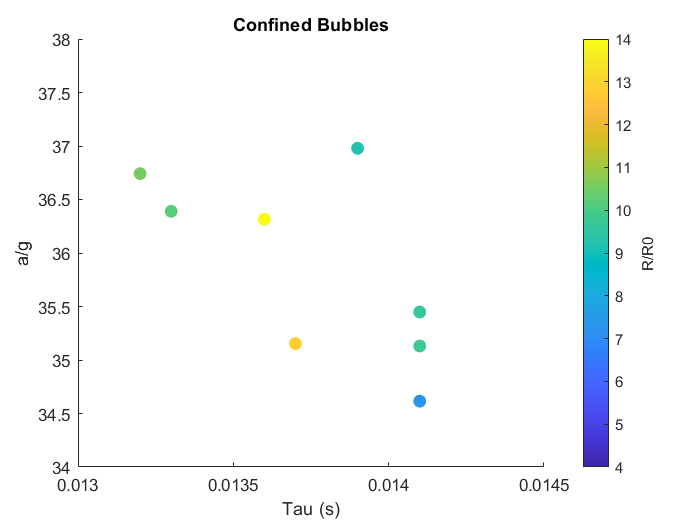
\includegraphics[width=\linewidth]{a_tau_conf.png}
    \caption{Confined Bubbles}
  \end{subfigure}
  \begin{subfigure}[b]{0.49\linewidth}
    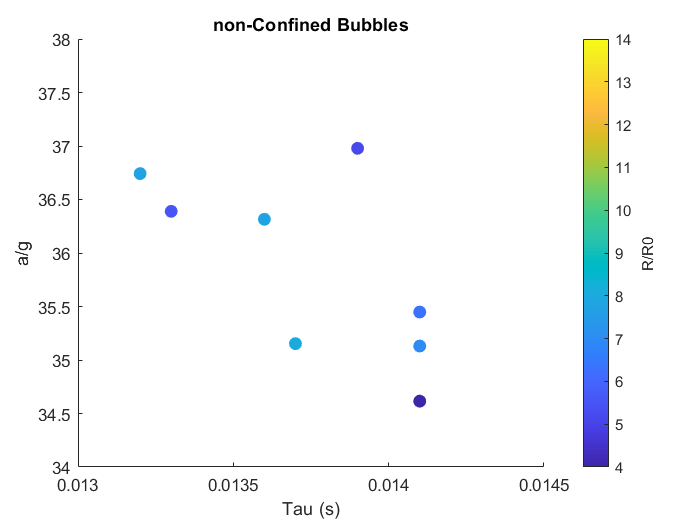
\includegraphics[width=\linewidth]{a_tau_nonconf.png}
    \caption{Non-Confined Bubbles}
  \end{subfigure}
  \caption{Comparison of Evolution of Radius with and without confinement}
\end{figure}
We can clearly see here that we have a difference in the evolution of the radius due to confinement, as the ratio $\frac{R}{R_0}$ indicated by the colour bar is much larger for the same acceleration and time in figure 2(a) than in figure 2(b). This difference can be seen even more clearly by comparing two bubbles at the same $a$ and $\tau$. This is done below using \emph{directcomp.m}.
\begin{figure}[H]
    \centering
    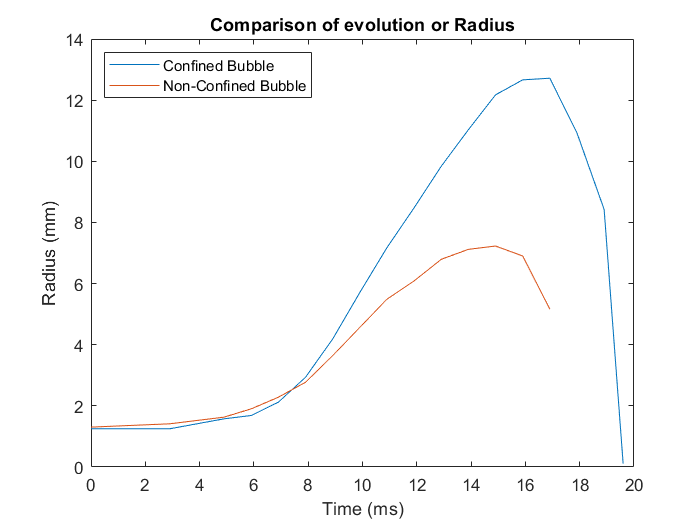
\includegraphics[width = 0.8\linewidth]{directcomp.png}
    \caption{Direct Comparison of the Evolution of the Radius}
\end{figure}
This very clearly reveals the difference in growth of the bubbles when confined and not.
\section{Questions Raised by first Tests}
The results above, while striking, raised a set of questions about unknowns within the experiment, namely:
\begin{enumerate}
    \item Do the bubbles interact between themselves?
    \item Is the non-confined bubble affected by the confining cylinder?
    \item What shape does the bubble take as it grows?
\end{enumerate}
We will address these question one by one. In order to answer the first question, a series of tests were performed comparing two unconfined bubbles, and one unconfined bubble. Below are the results, using the data sets \emph{confinement\_singlemiddle} and \emph{confinement\_interactmid}, and the script \emph{a\_tau\_comp\_mid.m}.
\begin{figure}[H]
  \centering
  \begin{subfigure}[b]{0.49\linewidth}
    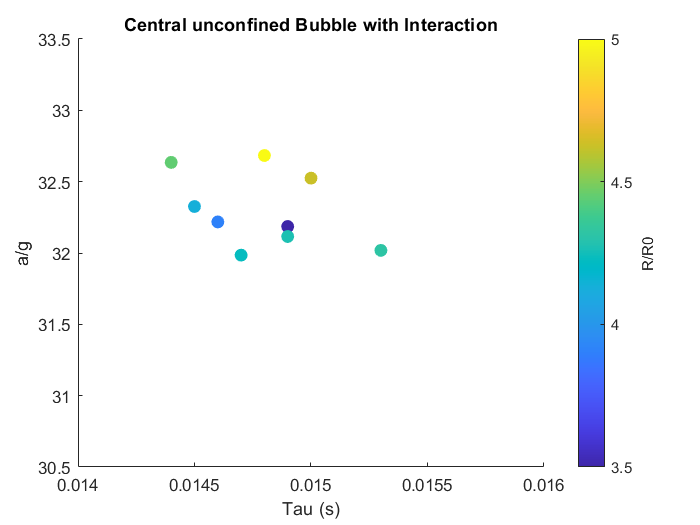
\includegraphics[width=\linewidth]{interact.png}
    \caption{Bubbles with interaction}
  \end{subfigure}
  \begin{subfigure}[b]{0.49\linewidth}
    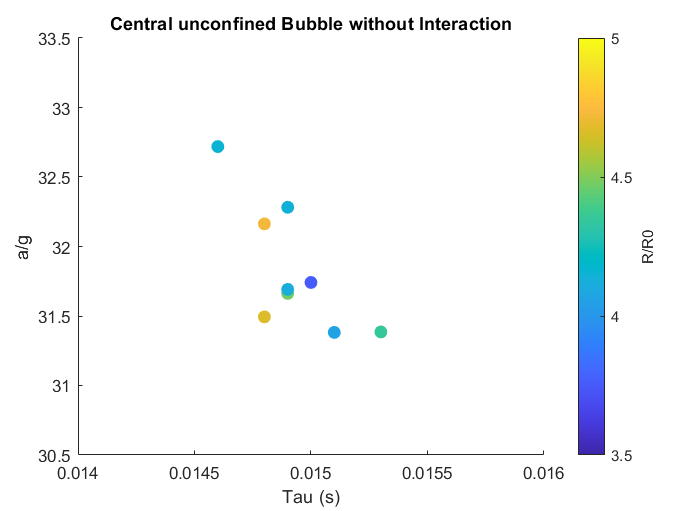
\includegraphics[width=\linewidth]{no_interact.png}
    \caption{Bubbles without interaction}
  \end{subfigure}
  \caption{Comparison of Evolution of Radius with and without interaction}
\end{figure}
Direct comparisons of figure 4(a) and figure 4(b) does not yield a lot of information, as it is difficult to reproduce exact \at characteristics from one drop to the next, however, comparisons of similar drops seemed to indicate that interaction had a slight damping effect on the growth of the bubble. This seems physically coherent, since the bubble growth induces a slightly increased pressure field around it, reducing the pressure difference seen by the other bubble.

In order to answer the second question, a series of tests was performed with one bubble on the side, with and without the confining cylinder, to understand whether its presence affected the non-confined bubble. Below are the results, using the data sets \emph{confinement\_interactedge} and \emph{confinement\_twoconfedge}, and the script \emph{a\_tau\_comp\_edge.m}.
\begin{figure}[H]
  \centering
  \begin{subfigure}[b]{0.49\linewidth}
    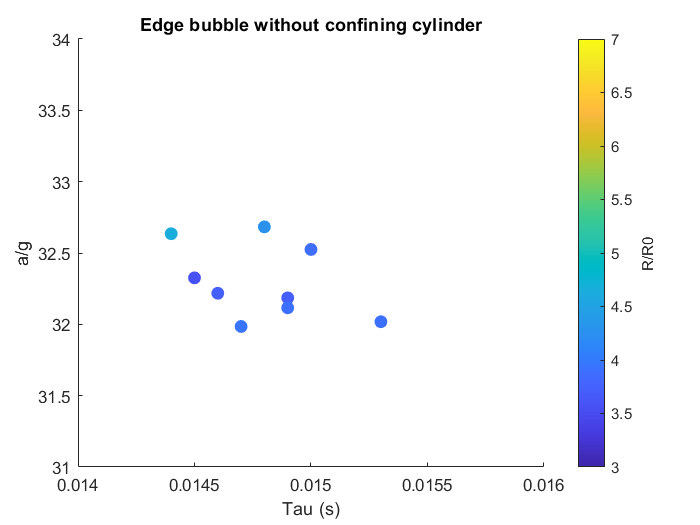
\includegraphics[width=\linewidth]{edgeconf.png}
    \caption{Bubbles without Confining Cylinder}
  \end{subfigure}
  \begin{subfigure}[b]{0.49\linewidth}
    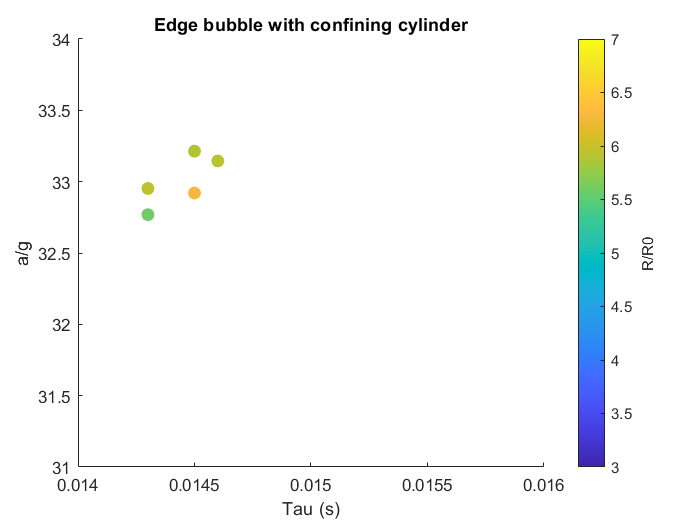
\includegraphics[width=\linewidth]{edgenoconf.png}
    \caption{Bubbles with Confining Cylinder}
  \end{subfigure}
  \caption{Comparison of Evolution of Radius with and without Confining Cylinder}
\end{figure}
Here the difference between figure 5(a) and figure 5(b), although the \at profile is slightly different, is clearer, and seems to indicate that the confining cylinder seems to increase the radius of the non-confined bubble. While this does not bring into question the conclusions reached in the first section, it does raise the question of what the actual amount of difference is between confined and non-confined bubbles is, caeteris paribus. In order to test this, the same experiment was performed several times with only one bubble, with and without confinement. The data used is \emph{confinement\_interactmid} and \emph{confinement\_twoconfmid}, and the script \emph{a\_tau\_comp\_conf.m}.
\begin{figure}[H]
  \centering
  \begin{subfigure}[b]{0.49\linewidth}
    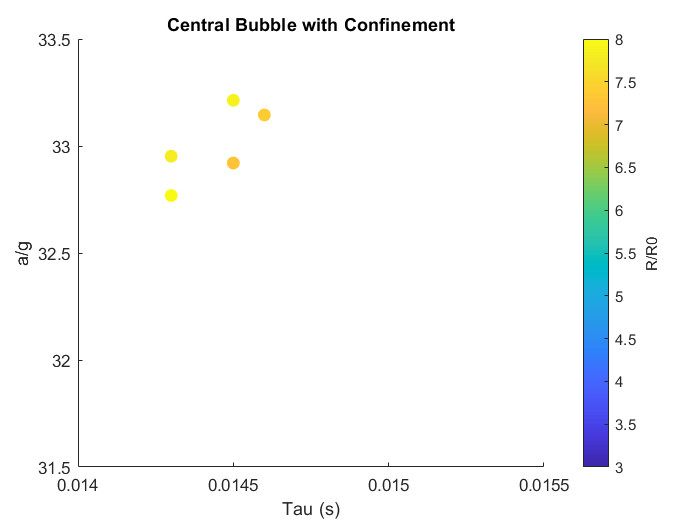
\includegraphics[width=\linewidth]{midconf.png}
    \caption{Bubbles with Confinement}
  \end{subfigure}
  \begin{subfigure}[b]{0.49\linewidth}
    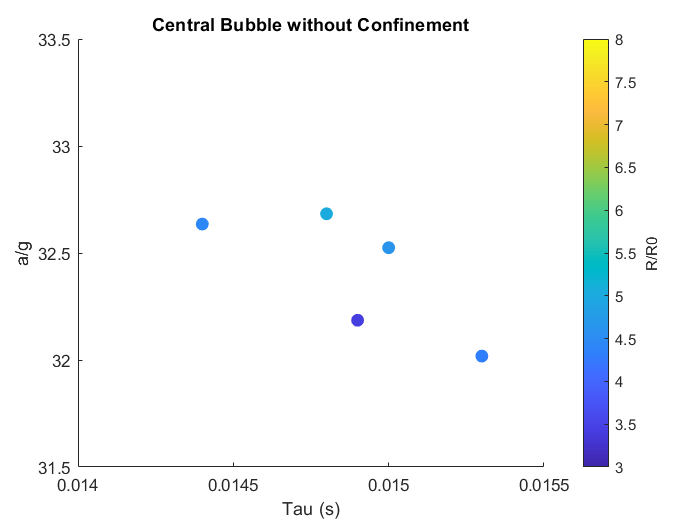
\includegraphics[width=\linewidth]{midnonconf.png}
    \caption{Bubbles without Confinement}
  \end{subfigure}
  \caption{Comparison of Evolution of Radius with and without Confinement}
\end{figure}
Despite the different positions on the \at diagram, we can clearly see the increased growth of the radius due to confinement.

\section{Determining Bubble Shape}


The answer to the final one of those three questions earns itself a section of its own for the monumental amount of time that it consumed. It was realised while running the first tests that the bubble may not have had the hemispherical shape initially assumed. In order to test this an additional camera was set up perpendicular to the drop. Several new lids also had to be built in order to be able to see the bubble from the top and the side. 

The first important observation is that there seem to be two regimes within which the experiment is operating, based on the size of the acceleration. Below 50g, we observe a simultaneous widening and flattening of the bubble (as can be observed in the figure on the title page). Above 50g, we observe a simultaneous widening and thickening of the bubble. Below are graphs of these two examples, using the data sets \emph{top\_nc}, \emph{cote\_nc}, \emph{HighCav\_top}, \emph{HighCav\_cote}, \emph{HighCav\_acc}, and the scripts \emph{ncplot.m} and \emph{highcavplot.m}.
\begin{figure}[H]
  \centering
  \begin{subfigure}[b]{0.49\linewidth}
    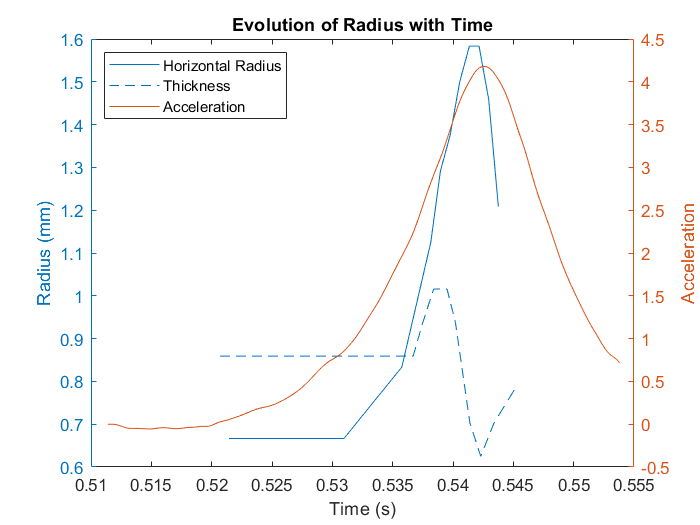
\includegraphics[width=\linewidth]{lowreg.png}
    \caption{Bubbles under 50g}
  \end{subfigure}
  \begin{subfigure}[b]{0.49\linewidth}
    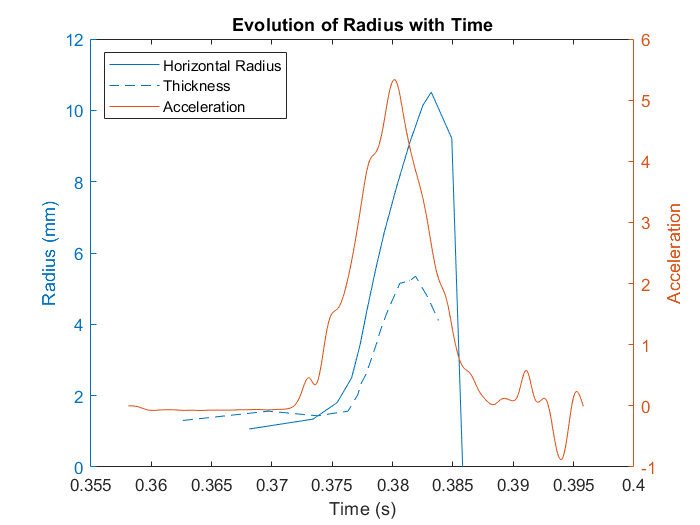
\includegraphics[width=\linewidth]{highreg.png}
    \caption{Bubbles over 50g}
  \end{subfigure}
  \caption{Comparison of Evolution of Radius in different regimes of Acceleration}
\end{figure}

\section{Confined vs Non-Confined Volume}

The final comparison that was possible at the very end of the internship was that of the volumes of bubbles under the high acceleration regime. By capturing video of the top and side, estimates of the volume of the bubbles became possible. However, due to the fact that the experiment was beginning to fall apart, and that the hermetic seals that guaranteed that no external air entered the cylinder had quite comprehensively abandoned their functions, only two reliable reading could be taken in the confined state. These two observations can nonetheless be compared with observations retrieved at similar \at values when unconfined to get an idea of the difference in the way the volume of the bubble evolves. In order to get the best match, \emph{HighCavConf\_1} ($a = 69.3, \tau = 5.5 \times 10^{-3}$) was compared with \emph{HighCav\_7} ($a = 63.5, \tau = 5.4 \times 10^{-3}$) and \emph{HighCavConf\_2} ($a = 52.4, \tau = 6.7 \times 10^{-3}$) was compared with \emph{HighCav\_2} ($a = 51.3, \tau = 6.9 \times 10^{-3}$), using the scriopt \emph{volumegraph.m}.
\begin{figure}[H]
  \centering
  \begin{subfigure}[b]{0.49\linewidth}
    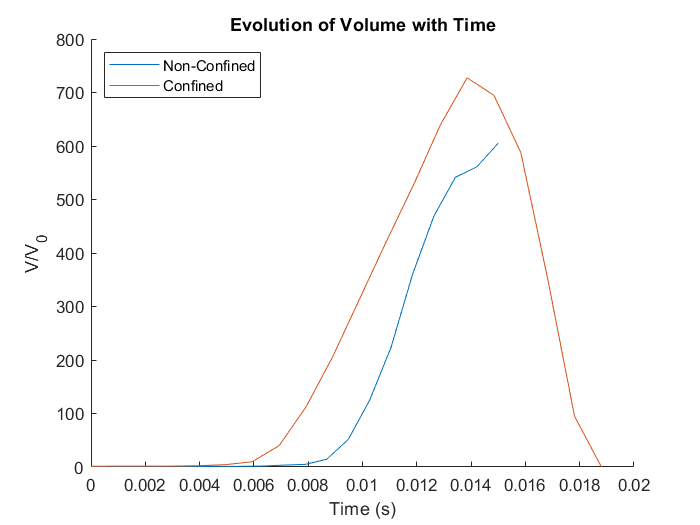
\includegraphics[width=\linewidth]{volumecomp1.png}
    \caption{\emph{HighCavConf\_1} compared with \emph{HighCav\_7}}
  \end{subfigure}
  \begin{subfigure}[b]{0.49\linewidth}
    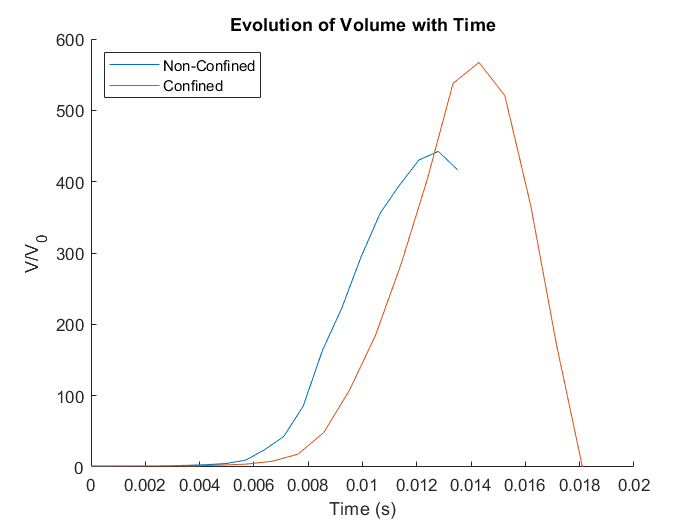
\includegraphics[width=\linewidth]{volumecomp2.png}
    \caption{\emph{HighCavConf\_2} compared with \emph{HighCav\_2}}
  \end{subfigure}
  \caption{Comparison of Evolution of Radius in different regimes of Acceleration}
\end{figure}
In order to calculate the volumes, we consider the bubbles to be hemi-ellipsoidal, such that their volume is $\frac{2}{3}\pi r^2e$, with $r$ the horizontal radius and $e$ the vertical radius or thickness of the bubble. However, in the case of confinement, when the bubble touches the confining cylinder, side videos show that it becomes relatively cylindrical, so at this point the volume is simply $\pi r^2e$. What these two figures show is that, at least for these cases, the volume increases more when confined than when not confined. Naturally, more data would have to be taken to confirm these findings.


\section{Pressure tests}
It is important to mention also the tests that were performed to understand the pressure at the lid of the cylinder. During tests with pressure sensors in one of the lids used for capturing side views of the bubble, inconsistencies led to further tests on the sensors themselves. Specifically, there was a question as to whether there was a radial dependence of the pressure at the lid, and if the pressure at the edge of the lid was higher than in the middle. However, after 2 weeks, it became clear that the sensors were in fact giving contradictory results, and as such they have been returned to the manufacturer for re-calibration. The radial dependency of the pressure is in direct contradiction with the physical observations obtained, which are that bubbles placed at any distance from the radius evolve in the same way, and therefore the pressure must be the same across the lid. I will not include the pressure data here since the sensors were unreliable and regularly disagreed with themselves. However, it can be found in the repository under the \emph{Pressure Tests} section, with the sensor and position labelled in the spreadsheet for each drop.

\section{Conclusion}

Overall, these results leave us with as many, if not more, questions than answers. The first big unanswered question pertains to the stratification of pressure within the cylinder. If the pressure was not stratified as we expected, it may well invalidate a large number of the results obtained above.

The second question is that of the volume. The results obtained above seem to show a slightly higher volume under confinement, but it is difficult to draw conclusions from such a small data set, and in particular one which we have observed to be very sensitive to initial conditions. Therefore, while they are not conclusive, they will likely serve as a useful base for experimentation with the new, and hopefully more reliable drop-tank.

It is also worth considering the conditions under which the assumptions that were made will hold, specifically with regards to the shape of the bubble under confinement. Here, in the high regime of acceleration, video evidence shows that the cylindrical treatment of the bubble is correct, however, we know from lower acceleration cases that the bubble does not necessarily touch the confining cylinder, and in those cases the volume is reduced by a factor of $\frac{2}{3}$ compared to the calculations made above. In future measurements, it will therefore likely be very useful to get side views of bubbles at a large range of accelerations, and for much smaller initial bubbles (potentially even no initial bubble), in order to best approximate brain-like conditions.

It would also be interesting to understand the reason behind the flattening of the bubble that is observed in low regimes.

\begin{figure}[H]
    \centering
    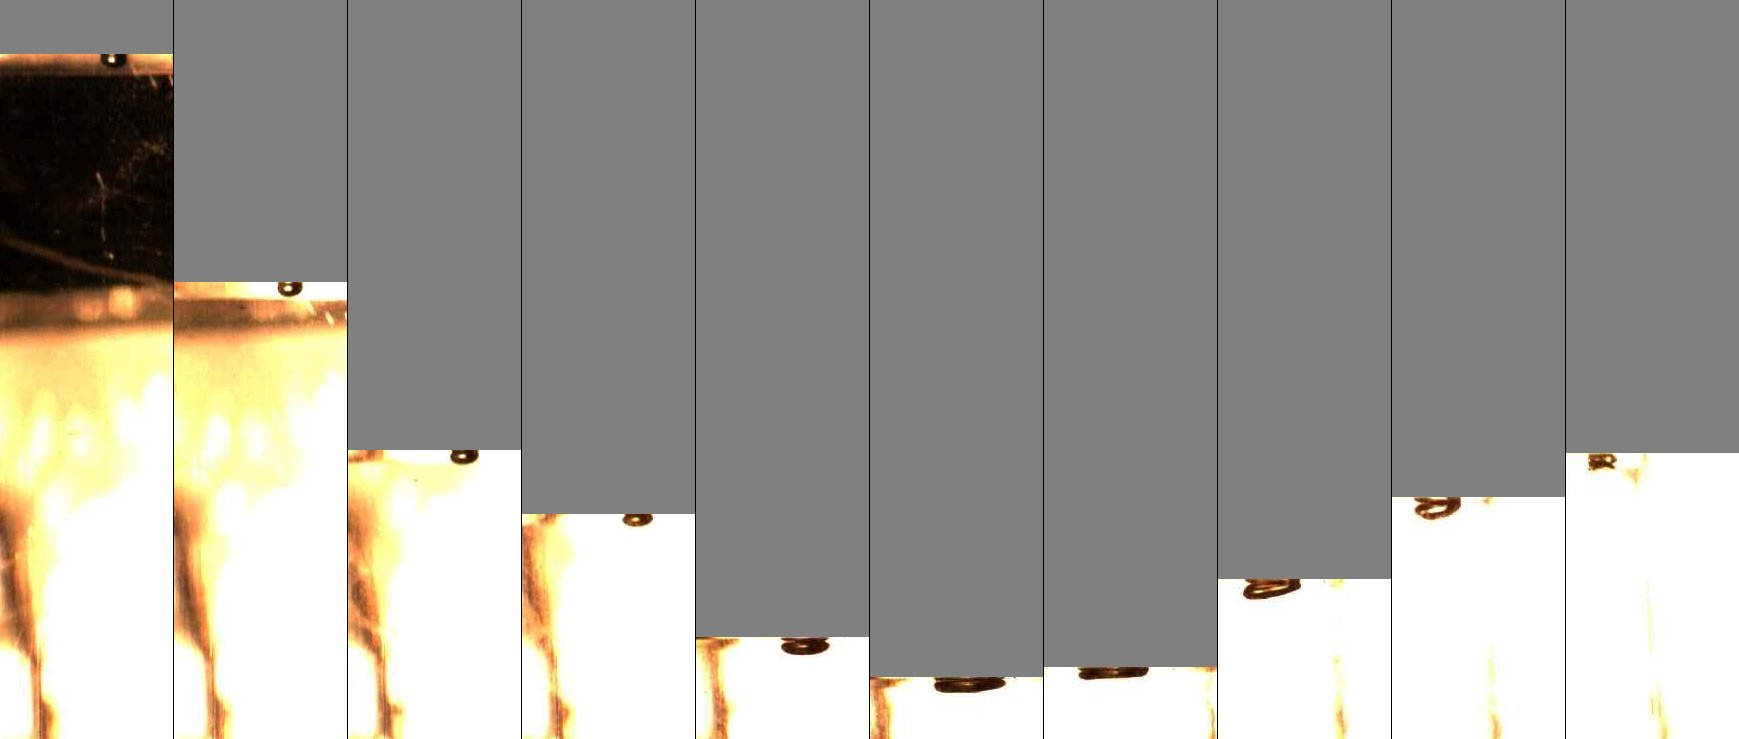
\includegraphics[width=\linewidth]{Montage3.jpg}
    \caption{Successive images of a single drop (\emph{cote\_nc\_4})}
\end{figure}
\end{document}

